\documentclass[openany]{book}
\usepackage[utf8]{inputenc}
\usepackage{verbatim}
\usepackage[hypertexnames=false]{hyperref}
\usepackage{amstext} 
\usepackage{array}   
\newcolumntype{C}{>{$}c<{$}} 


\input{structure}
\usepackage{geometry}
\geometry{
    top=3cm,
    bottom=3cm,
    left=3cm,
    right=3cm,
    headheight=14pt, 
    footskip=1.4cm,
    headsep=10pt,
}
\usepackage{graphicx}
\title{Delirios de AnalFun}
\author{Paco Mora}
\date{\today}

\begin{document}

\maketitle

\chapter{Yo qué sé qué es esto}

\begin{definition}
    
    Un espacio de medida nula de primera categoría cuando está contenido en una unión numerable de cerrados con interior vacío. Si no es de primera categoría se llama de segunda categoría.
\end{definition}


\begin{theorem}
    \textbf{(Baire)}    

    Sea $ (X,d) $ espacio métrico completo $ \{G_n\}_{n \in \mathbb{N}} $ abiertos de en $ X $, $ \overline{G}_{r} = X\ \forall n \in N $. Entonces:
    $$ \bigcap_{n=1}^{\infty}G_n \ne \emptyset $$
\end{theorem}

\textit{\textbf{//Repaso de la relación de orden}}

\begin{theorem}
    \textbf{Principio de la buena ordenación }
    Para todo conjunto $ \mathcal{S}   $, existe una relación de orden $ \leq  $ tal que $ (S, \leq ) $ está bien ordenado, $ \leq  $ es un buen orden.
\end{theorem}


\begin{theorem}
    \textbf{Lema de Zorn}

    Si $ (P,\leq ) $ es un conjunto parcialmente ordenado en el que cada cadena tiene una cota superior (para $ C $, cadena, existe $ c \in P $ tal que $ x\leq c $ para todo $ x \in C $), entonces $ P $ tiene un elemento maximal (existe $  m \in P $ tal que si $ \leq x $ entonces $ x = m $)
\end{theorem}

\begin{theorem}
    \textbf{Principio Maximal de Hasudorff}

    Cada conjunto parcialmente ordenado ($ P,\leq  $) contiene una cadena maximal.

\end{theorem}

\newpage
\begin{theorem}
    Son equivalentes:
    \begin{enumerate}
        \item El principio Maximal de Hasudorff
        \item Lema de Zorn
        \item Principio de la buena ordenación
        \item Axioma de elección
    \end{enumerate}
\end{theorem}

//Definiciones de espacio de Hilbert y de Banach


//1.2.8 del libro

//Del 1.3 ha dicho que lo leamos.

//"Los teoremas que pregunto son los que tienen nombre"


\begin{theorem}
    \textbf{De la mejor aproximación}

    Dado $ (H,<\cdot >) $ espacio de Hilbert y $ C \subset H $ cerrado y convexo. Sea $ x_0 \not  \in C $. Entonces existe un único elemento $ c_0 \in C $ tal que $ \|x_0-x\| = \inf \{\|x_0-c\|\ = \alpha :\ c \in C\} $

\end{theorem}

\begin{demonstration}
    Tomemos una sucesión $(c_n)_{n \in \mathbb{N}}$ con $ c_n \in C $ de forma que se verifique 

    %imagen

    \begin{tikzpicture}
        \draw[black, very thick] (0,0) rectangle (4,0);
        \node[circle,inner sep=1pt,fill=red,label={$\alpha$}] at (1,0) {};
        \node[circle,inner sep=1pt,fill=red,label={$\|c_n\|$}] at (2,0) {};
        \node[circle,inner sep=1pt,fill=red,label={$\alpha +\dfrac{1}{n}$}] at (3,0) {};
    \end{tikzpicture}

    Si $ c_n $ fuera de Cauchy, existe $ c_0 = \lim_{n \to \infty} c_n $. Probemos que $ (c_n) $ es de Cauchy. Para ello basta usar la identidad del paralelogramo.

    Como $ \underbrace{2\|c_n\|^2}_{2 \alpha ^2}+ \underbrace{2\|c_m\|^2}_{2 \alpha ^2}-\|c_n+c_m\|^2 = \|c_n-c_m\|^2 $

    Dividimos la expresión por 4 podemos usar la convexidad de $ C $ para el punto medio entre $ c_n $ y $ c_m $:
    $$ \dfrac{1}{2}\|c_n\|^2 + \dfrac{1}{2}\|c_m\|^2 - \left\|\dfrac{c_n+c_m}{2}\right\| ^2= \dfrac{1}{4}\|c_n-c_m\|^2 $$

    Ahora tomamos límites para ver que $ \|c_n-c_m\| \to 0 $.

\end{demonstration}

\begin{theorem}
    \textbf{(de la proyección)}    

    Sea $ M  $ un subespacio cerrado del Hilbert $ H $, entonces existen un único par de aplicaciones lineales continuas $ P,Q: H \to H $ tales que $ P(H) = M $ y $ Q(H) = M^{\perp } = \{y \in H:\ <y,m> = 0\ \forall  m \in M\} $ y $ x = Px+Qx\ \forall x \in H $

    Además se verifica:
    \begin{itemize}
        \item $ x \in M \implies Px =x,\ Qx = 0;\ x \in M ^{\perp} \implies Px = 0,\ Qx = x $
        \item $ \|x-Px\| = \inf \{\|x-y\|,\ y \in M\}\ \forall x \in H $
        \item $ \|x\|^2 = \|Px\|^2+\|Qx\|^2 $ (Pitágoras)
    \end{itemize}

    Como consecuencia $ H = M \oplus M^{\perp} $
\end{theorem}

\begin{demonstration}

    Sea $ x \in H,\ x+M $ cerrado y convexo, llamemos $ Qx $ alúnico elemento en $ x+M $ de norma mínima y definimos $ Px = x-Qx $. Vemos que $ Qx \in M^{\perp} $, $ <z,y> = 0 \forall y \in M $. Aplicando que $ Qx \equiv Z $ tiene norma mínima en $ x+M $ tendremos:
    $$ 0\leq  \|z\|^2 = <z,z> \leq  \underbrace{\|z-\alpha y\|^2}_{ \forall \alpha \in \mathbb{R}} = <z-\alpha y,z-\alpha y> = \cancel{<z,z>} - \overline{\alpha}<z,y> - \alpha <y,z> = \alpha ^2\|y\|^2  $$
    
    Tomando ahora $ \alpha = <z,y>  $ y como se tiene que cumplir siempre que la expresión es mayor o igual que 0 llegamos a $ 0 \leq  -\alpha ^2 \implies \alpha = 0 $, luego $ \operatorname{Im}(Q) \subset H^{\perp} $. Como además $ M \cap M^{\perp} = \{0\} \implies x = Px+Qx $, entonces $ H = M \oplus M^{\perp} $

    Análogamente sale el resto de los enunciados\footnote{xd}.

\end{demonstration}

\begin{lemma}
    $ M \subset H $ subespacio estricto cerrado del espacio de Hilbert H. Entonces $ \exists x_0 \ne 0, x_0 \perp M $, $ <x_0,m\geq 0 \forall m \in M $

\end{lemma}
\begin{demonstration}

    Como $ H \ne M \implies M ^{\perp} \ne \{0\} $
    $$ \{d_n:\ n=1,2,..\} \text{numerable y denso en }H$$
    
    Tomamos entonces una base ortonormal $ \{e_1,e_2,...,e_n,...\} $ tal que:
    $$ \operatorname{span} \{d_1,...,d_n,...\} = \operatorname{span} \{e_1,...,e_n,...\} $$
\end{demonstration}
    
    \begin{definition}
        
        \textbf{Conjunto ortonormal} $ \{\overline{u}_1,\overline{u_2},...\} $ en $ H:\ <u_i,u_j> = \delta_{ij} $. Tenemos además que son LI:
        $$ 0 = \|\sum\limits_{i=1}^{n}c_i 0_{i}\|^2 = <\sum\limits_{i=1}^{n}c_i 0_{i},\sum\limits_{i=1}^{n}c_i 0_{i}> = \sum\limits_{i=1}^{n}c_i^2 \implies c_i = 0,\ i=1,2,...,n$$
    \end{definition}

    \begin{proposition}
        $ M = \operatorname{span} \{u_1,u_2,...,u_n\} \subset H,\ P_{M}(x) = \sum\limits_{i=1}^{n}<x_i,u_i>u_i$. Si $ d = dist \{x,M\} $ entonces:
        $$ \|x\|^2 - \delta ^2 = \sum\limits_{i=1}^{n}|<x,u_i>|^2 $$
    \end{proposition}

    \begin{lemma}
        Sea $ \{u_1,u_2,...,u_n,...\} $ ortonormal, $ \|x\|^2 \geq \sum\limits_{i=1}^{\infty} |<x,u_i>|^2\ \forall x \in H$
    \end{lemma}
\newpage
\begin{proposition}
    $ \{u_1,u_2,...,u_n,...\} $ ortonormal en $ H $, la función:
    $$ \Lambda: H \to \ell^2\ \Lambda(x) = \left( <x,u_i>   \right)_{i=1}^{\infty} $$
    es continua y sobre
\end{proposition}

\begin{demonstration}
    $ (\xi_n) \in \ell ^2 $ encontramos $ x \in H $: $ \Lambda(x) = (\xi_n) $. Nos preguntamos si:
    $$ \sum\limits_{i=1}^{\infty} \xi_nu_n \to <\sum\limits_{n=1}^{\infty}\xi_nu_n,u_m> $$

    No se ve nada en la pizarra, ha probado que es de Cauchy para ver que es convergente.

\end{demonstration}

\begin{theorem}
    \textbf{(de la base hilbertiana)}

    Para $ \{u_1,u_2,...,u_n,...\} $ conjunto ortonormal en $ H $ (espacio de Hilbert). Son equivalentes:
    \begin{enumerate}
        \item $ \{u_1,u_2,...\} $ es ortonormal maximal.\vspace{3mm}
        \item $ \overline{\operatorname{span} \{u_1,...\}} = H $
        \item $ \forall x \in H $ se tiene $ x = \sum\limits_{n=1}^{\infty}<x,u_n>u_n $ en $ H $
        \item $ \forall x \in H,\ \forall y \in H $, se tiene $ <x,y> = \sum\limits_{n=1}^{\infty}<x,u_n>\overline{<y,u_n>} $
        \item $ \forall x \in H $, se tiene $ \|x\|^2 = \sum\limits_{n=1}^{\infty}|<x,u_n>|^2 $

    \end{enumerate}
    A la igualdad de los dos últimos puntos se le llama Identidad de Parseval
\end{theorem}

\begin{demonstration}
    Te la miras en el libro, crack. (puede entrar en el examen)
\end{demonstration}

\begin{definition}
    A una base como la anterior se le llama \textbf{base hilbertiana}. A los coeficientes se les llama coeficientes de Fourier.
\end{definition}


\end{document}

